\documentclass{standalone}
\usepackage{tikz}
\usetikzlibrary{matrix, positioning, shapes, arrows, calc}

\tikzset{>=latex}

\begin{document}

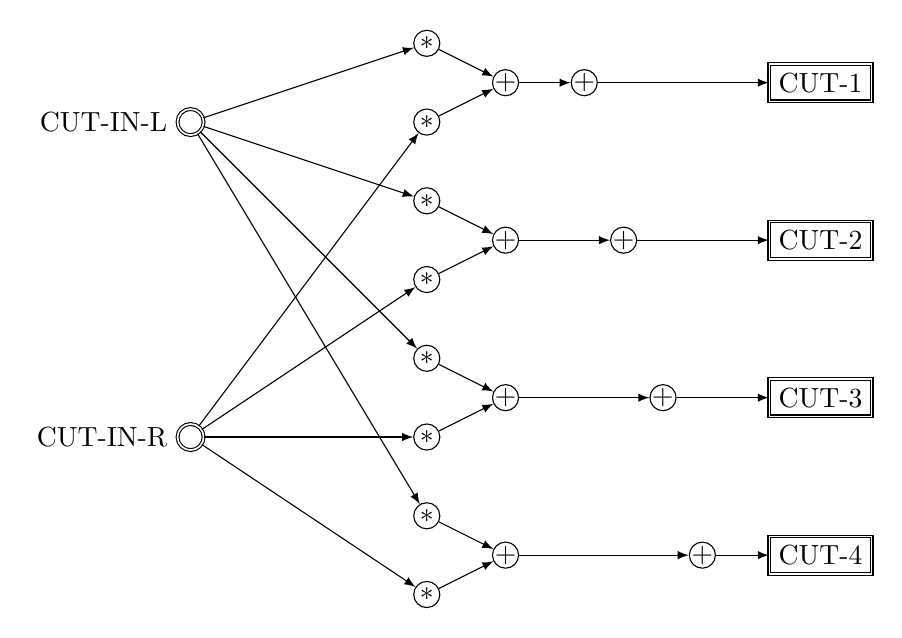
\begin{tikzpicture}

\tikzstyle{input}=[draw=black, circle, double, minimum size=1]
\tikzstyle{output}=[draw=black, circle, double, minimum size=1, fill=gray!40]
\tikzstyle{mul}=[draw=black, circle, minimum size=1, label=center:$\ast$]
\tikzstyle{add}=[draw=black, circle, minimum size=1, label=center:$+$]
\tikzstyle{or}=[draw=black, circle, minimum size=1, label=center:$|$]
\tikzstyle{param}=[draw=black, rectangle, dotted, thick]
\tikzstyle{bus}=[draw=black, rectangle, double]


% inputs
\node [input, label=left:CUT-IN-L] (in-l) at (0, 10) {};
\node [input, label=left:CUT-IN-R] (in-r) at ($(in-l) - (0, 4)$) {};

\node [mul] (in-l-mul-1) at ($(in-l) + (3, 1)$) {};
\node [mul] (in-r-mul-1) at ($(in-l-mul-1) +(0, -1)$) {};
\node [mul] (in-l-mul-2) at ($(in-r-mul-1) +(0, -1)$) {};
\node [mul] (in-r-mul-2) at ($(in-l-mul-2) +(0, -1)$) {};
\node [mul] (in-l-mul-3) at ($(in-r-mul-2) +(0, -1)$) {};
\node [mul] (in-r-mul-3) at ($(in-l-mul-3) +(0, -1)$) {};
\node [mul] (in-l-mul-4) at ($(in-r-mul-3) +(0, -1)$) {};
\node [mul] (in-r-mul-4) at ($(in-l-mul-4) +(0, -1)$) {};

\draw [->] (in-l) -- (in-l-mul-1);
\draw [->] (in-l) -- (in-l-mul-2);
\draw [->] (in-l) -- (in-l-mul-3);
\draw [->] (in-l) -- (in-l-mul-4);
\draw [->] (in-r) -- (in-r-mul-1);
\draw [->] (in-r) -- (in-r-mul-2);
\draw [->] (in-r) -- (in-r-mul-3);
\draw [->] (in-r) -- (in-r-mul-4);

% voices
\node [add] (voice-in-1) at ($(in-l-mul-1) + (1, -0.5)$) {};
\node [add] (voice-in-2) at ($(voice-in-1) + (0, -2)$) {};
\node [add] (voice-in-3) at ($(voice-in-2) + (0, -2)$) {};
\node [add] (voice-in-4) at ($(voice-in-3) + (0, -2)$) {};
\node [add] (voice-in-fb-1) at ($(voice-in-1) + (1, 0)$) {};
\node [add] (voice-in-fb-2) at ($(voice-in-2) + (1.5, 0)$) {};
\node [add] (voice-in-fb-3) at ($(voice-in-3) + (2, 0)$) {};
\node [add] (voice-in-fb-4) at ($(voice-in-4) + (2.5, 0)$) {};
\foreach \i in {1,...,4}
{
	\node [bus] (voice-\i) at ($(voice-in-\i) + (4, 0)$) {CUT-\i};
	\draw [->] (in-l-mul-\i) -- (voice-in-\i);
	\draw [->] (in-r-mul-\i) -- (voice-in-\i);
	\draw [->] (voice-in-\i) -- (voice-in-fb-\i);
	\draw [->] (voice-in-fb-\i) -- (voice-\i);
}

%\node [bus] (voice-2) at ($(voice-in-2) + (2, 0)$) {VOICE-2};
%\node [bus] (voice-3) at ($(voice-in-3) + (2, 0)$) {VOICE-3};
%\node [bus] (voice-4) at ($(voice-in-4) + (2, 0)$) {VOICE-4};

%\draw [->] (in-l-mul-1) -- (voice-in-1);
%\draw [->] (in-r-mul-1) -- (voice-in-1);

\end{tikzpicture}
\end{document}
